\section{Variational Quantum Eigensolver}
References: \cite{Anand2021}, \cite{McClean2016}, \cite{Chan2021}

\subsection{Unitary Coupled Cluster}

Whilst unitary coupled cluster theory was proposed in X, interest in its applications has been minimal due to the inability of classical computers to efficiently evaluate its equations. As suggested by Peruzzo et al \cite{Peruzzo2014}, the UCC formulation of a wavefunction can be efficiently implemented on a quantum computer using quantum gates.

Unitary coupled cluster theory allows us to represent an arbitrary state $\ket\psi$ using the following exponential ansatz.
\begin{equation*}
    \ket\psi = e^{\hat T(\mathbf{\theta}) - \hat T^\dagger(\mathbf{\theta})} \ket{\psi_0}
\end{equation*}

Where $\ket{\psi_0}$ is a single reference Slater determinant, usually the Hartree-Fock groundstate obtained via the self-consistent field method. The exponential operator $U(\theta) = e^{\hat T(\mathbf{\theta}) - \hat T^\dagger(\mathbf{\theta})}$ is unitary since its exponent $\hat T(\mathbf{\theta}) - \hat T^\dagger(\mathbf{\theta})$ is anti-Hermitian.

The excitation operators are given by
\begin{equation*}
\hat T(\mathbf{\theta}) - \hat T^{\dagger}(\mathbf{\theta}) =
\sum_{i, a} \theta^a_i (a^\dagger_i a_a - a^\dagger_a a_i) + 
\sum_{i, j, a, b} \theta^{ab}_{ij} (a^\dagger_i a^\dagger_j a_a a_b - a^\dagger_a a^\dagger_b a_i a_j) + \dots
\end{equation*}

Where $i, j$ indexes occupied spin orbitals and $a, b$ indexes virtual, or unoccupied, spin orbitals. The resulting unitary operator $U(\theta)$ cannot be directly implemented on a quantum computer since the terms of the excitation operator do not commute. Instead, we must invoke the Trotter formula to approximate the unitary.

\begin{equation*}
    e^{A+B} = (e^A \, e^B)^\rho
\end{equation*}

Taking a single Trotter step $\rho=1$, we obtained the disentangled UCC
\begin{equation}
    U_{t1}(\mathbf\theta) = \prod_m e^{\theta_m (\tau_m - \tau_m^\dagger)}
\end{equation}

Where $m$ indexes all possible excitations. It has been shown in \cite{Evangelista2019} that the disentangled UCC can exactly parametrise any state.

"In practice, the excitations are truncated to only include single and double excitations. This UCCSD ansatz has been popular in the VQE literature and is often the benchmark for more cost effective methods." \cite{Chan2021}.

"Only UCCSD excitation operators which conserve spin were
used for ansatz construction. Ansatze generated in this manner
preserve the spin symmetry of the spin reference" \cite{Chan2021}

---

In this chapter we introduce we introduce Unitary Coupled Cluster theory which will serve as the basis for the Variational Quantum Eigensolver algorithm introduced in chapter XXX. In particular, we are interested in developing the Unitary-Product State which will serve as a variational ansatz.

% Despite advances in quantum computing hardware and software, many quantum algorithms require resources not yet available to us...

% Original paper introducing VQE is McClean

One notable advantage of the VQE algorithm is its ability to be run on any quantum architecture, moreover, we can leverage architecture requirements when designing the variational ansatz. \cite{McClean2016}.

"Even in the event that some error correction is required to exceed current computational capabilities, this same robustness may translate to requiring minimal error cor- rection resources when compared with other algorithms." \cite{McClean2016}

We begin by...


%%%

Within the traditional coupled-cluster framework, the ground electronic state is prepared by applying the CC operator to a reference state (usually Hartree-Fock).
\begin{equation*}
    \ket\psi = e^{\hat T} \ket{\phi_0}
\end{equation*}

Where $\hat T$ is the cluster excitation operator.

Quantum gates, however, must be unitary operators, so instead, we work within the UCC framework.

\begin{equation*}
    \ket\psi = e^{\hat T} \ket{\phi_0}
\end{equation*}

Where $\hat T$ is now an \textbf{anti-Hermitian} operator, and $e^{\hat T}$ is unitary.

In general, we can prepare exact electronic states by applying a sequence of $k$ parametrised unitary operators to our reference state.

\begin{equation*}
\begin{gathered}
    \ket\psi = \prod_i^k U_i(\theta_i) \ket{\phi_0} \\
    \text{Where $U_i(\theta_i)$ is a parametrised unitary operator}
\end{gathered}
\end{equation*}\smallskip

The parameters $\theta_i$ are then optimised to find the ground state energy.

General fermionic single and double excitation operators are defined as,
\begin{equation*}
    a_q^\dagger a_p \text{ and } a_r^\dagger a_s^\dagger a_q a_p
\end{equation*}

Exciting one electron from $p$ to $q$, and two electrons from $p, q$ to $r, s$ respectively.

Taking a linear combination of these, we obtain \textbf{anti-Hermitian} fermionic single and double excitation operators.
\begin{equation*}
\begin{gathered}
    \hat\kappa_p^q = a_q^\dagger a_p - a_p^\dagger a_q \\
    %
    \hat\kappa_{pq}^{rs} =
    a_r^\dagger a_s^\dagger a_q a_p - a_p^\dagger a_q^\dagger a_s a_r
\end{gathered}
\end{equation*}\smallskip

Such that upon exponentiating, we obtain \textbf{unitary} operators.

\begin{equation*}
    U^q_p = e^{\hat\kappa_p^q} \qquad
    %
    U_{pq}^{rs} = e^{\hat\kappa_{pq}^{rs}}
\end{equation*}

\subsection{\label{fermion-qubit-encodings}Jordan-Wigner Transformation}
References: \cite{Seeley2020}

The form of the occupation number representation vector and the qubit statevector suggests the following identification between electronic states and qubit states.
\begin{equation*}
    \ket{f_{n-1} \dots f_{0}} \quad\rightarrow\quad \ket{q_{n-1} \dots q_{0}}
\end{equation*}
That is, we allow each qubit to store the occupation number of a given spin-orbital. Hence, in order to actually simulate a Hamiltonian we must map the fermionic creation and annhilation operators onto qubit operators, and these operators must behave in the same way as their fermionic analogues.
\begin{equation*}
    \hat Q^+ \ket 0 = \ket 1 \qquad
    \hat Q^+ \ket 1 = 0 \qquad
    \hat Q \ket 1 = \ket 0 \qquad
    \hat Q \ket 0 = 0
\end{equation*}
The qubit operators must also preserve the fermionic anti-commutation relations in order to satisfy the Pauli antisymmetry requirement.
\begin{equation*}
    \{ \hat Q_{j}, \hat Q_{k} \} = 0 \qquad
    \{ \hat Q_{j}^{\dagger}, \hat Q_{k}^{\dagger} \} = 0 \qquad
    \{ \hat Q_{j}, \hat Q_{k}^{\dagger} \} = \delta_{jk}
\end{equation*}

One such qubit encoding is known as the Jordan-Wigner transformation. It expresses the fermionic creation and annhilation operators as a linear combination of the Pauli matrices.
\begin{equation*}
    \hat Q^+ = \ket 1 \bra 0 = \frac{1}{2} (X - iY) \qquad \hat Q = \ket 0 \bra 1 = \frac{1}{2} (X + iY) 
\end{equation*}

When dealing with \textbf{multiple-qubits}, we must also account for the occupation parity of the qubits preceding the target qubit $j$.
\begin{equation*}
    a_j^\dagger \ket{f_{n-1} \dots f_{j+1},\,\, 0,\,\, f_{j-1} \dots f_0} = (-1)^{\sum_{s=0}^{j-1} f_s} \ket{f_{n-1} \dots f_{j+1},\,\, 1,\,\, f_{j-1} \dots f_0}
\end{equation*}
We do this by introducing a string of Pauli Z operators that computes the parity of the qubits preceding the target qubit.
\begin{equation*}
\begin{gathered}
    \hat a_j^+ = \frac{1}{2} (X - iY) \prod_{k=1}^{j-1} Z_k \qquad
    \hat a_j = \frac{1}{2} (X + iY) \prod_{k=1}^{j-1} Z_k \\[2ex]
    \text{Where $\prod$ is the tensor product.}
\end{gathered}
\end{equation*}

A more compact notation is,
\begin{equation*}
    \hat a_j^+ = \frac{1}{2} (X - iY) \otimes Z^\rightarrow_{j-1} \qquad
    \hat a_j = \frac{1}{2} (X + iY) \otimes Z^\rightarrow_{j-1}
\end{equation*}
Where $Z^\rightarrow_{i}$ is the parity operator with eigenvalues $\pm 1$, and ensures the correct phase is added to the qubit state vector.
\begin{equation*}
    Z^\rightarrow_{i} = Z_i \otimes Z_{i-1} \otimes \dots \otimes Z_0
\end{equation*}
For instance, the creation operator $a^\dagger_3$ maps to the following Pauli string,
\begin{align*}
    \hat a_3^\dagger &=
    \frac{1}{2} (X_3 - iY_3) \otimes Z_2 \otimes Z_1 \otimes Z_0 \\
    %
    \hat a_3^\dagger &=
    \frac{1}{2} ( X_3 \otimes Z_2 \otimes Z_1 \otimes Z_0 ) -
    \frac{1}{2} i ( Y_3 \otimes Z_2 \otimes Z_1 \otimes Z_0 )
\end{align*}
Usually we drop the subscript specifying the orbital acted on.

\subsection{Excitation Operators}

Recalling the Jordan-Wigner encoding for the creation and annhilation operators,
\begin{equation*}
    \hat a_j^+ = \frac{1}{2} (X - iY) \otimes Z^\rightarrow_{j-1} \qquad
    \hat a_j = \frac{1}{2} (X + iY) \otimes Z^\rightarrow_{j-1}
\end{equation*}
The anti-Hermitian fermionic single and double excitation operators $\kappa_p^q$ and $\kappa_{pq}^{rs}$
\begin{align*}
    F_p^q = \frac{i}{2} & (Y_p X_q - X_p Y_q) \prod_{k=p+1}^{q-1} Z_k \\
    %
    F_{pq}^{rs} = \frac{i}{8} (
      & X_p X_q Y_s X_r +
        Y_p X_q Y_s Y_r +
        X_p Y_q Y_s Y_r +
        X_p X_q X_s Y_r - \\
      & Y_p X_q X_s X_r -
        X_p Y_q X_s X_r -
        Y_p Y_q Y_s X_r -
        Y_p Y_q X_s Y_r )
    \prod_{k=p+1}^{q-1} Z_k
    \prod_{l=r+1}^{s-1} Z_l
\end{align*}
Multiplying by $\theta$ and exponentiating yields the parametrised unitary qubit operators,
\begin{equation*}
    U^q_p (\theta) =
    \text{exp} \left( i
    \frac{\theta}{2} (Y_p X_q - X_p Y_q) \prod_{k=p+1}^{q-1} Z_k \right)
\end{equation*}

\begin{equation*}
    U^{rs}_{pq} (\theta) = \text{exp} \left( i \frac{\theta}{8} (
    X_p X_q Y_s X_r
    + \dots -
    Y_p Y_q Y_s X_r -
    Y_p Y_q X_s Y_r )
    \prod_{k=p+1}^{q-1} Z_k
    \prod_{l=r+1}^{s-1} Z_l
    \right)
\end{equation*}
To summarise, we constructed anti-Hermitian single and double excitation operators from a linear combination of fermionic excitation operators,
\begin{equation*}
    \hat\kappa_p^q = a_q^\dagger a_p - a_p^\dagger a_q \qquad
    %
    \hat\kappa_{pq}^{rs} =
    a_r^\dagger a_s^\dagger a_q a_p - a_p^\dagger a_q^\dagger a_s a_r
\end{equation*}\smallskip
We then mapped these to qubit operators using the Jordan-Wigner transformation,
\begin{equation*}
    \hat\kappa_p^q \xrightarrow{\text{JW}} F_p^q \qquad\qquad
    \hat\kappa_{pq}^{rs} \xrightarrow{\text{JW}} F_{pq}^{rs}
\end{equation*}
And finally, we exponentiated to yield the parametrised unitary qubit operators.
\begin{equation*}
    U^q_p (\theta) = e^{\theta^q_p F_p^q} \qquad
    %
    U^{rs}_{pq}(\theta) = e^{\theta_{pq}^{rs} F_{pq}^{rs}}
\end{equation*}

Let's look again at the parametrised single-body unitary operator,
\begin{equation*}
\begin{gathered}
    U^q_p (\theta) =
    \text{exp} \left( i
    \frac{\theta}{2} (Y_p X_q - X_p Y_q) \prod_{k=p+1}^{q-1} Z_k \right) \\
    %
    U^q_p (\theta) =
    \left( \text{exp} \left[
    i \frac{\theta}{2} Y_p X_q \prod_{k=p+1}^{q-1} Z_k \right] \right)
    %
    \left( \text{exp} \left[ -
    i \frac{\theta}{2} X_p Y_q \prod_{k=p+1}^{q-1} Z_k \right] \right)
\end{gathered}
\end{equation*}

The first exponential term can be implemented by the following phase gadget.
\begin{equation*}
    \text{exp} \left( i
    \frac{\theta}{2} Y_p X_q \prod_{k=p+1}^{q-1} Z_k \right)
\end{equation*}

\begin{figure}[H]
\centering
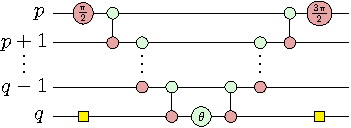
\includegraphics[width=8cm]{chapter-3/yx_cnot}
\end{figure}

Left CNOT ladder construction calculates the parity of the qubit state, and applies a rotation in the $Z$ basis if the parity is odd.

Whilst the second exponential term can be implemented by the phase gadget.
\begin{equation*}
    \text{exp} \left( - i
    \frac{\theta}{2} X_p Y_q \prod_{k=p+1}^{q-1} Z_k \right)
\end{equation*}

\begin{figure}[H]
\centering
    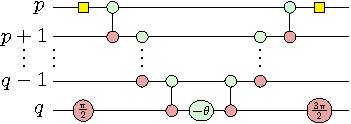
\includegraphics[width=8cm]{chapter-3/xy_cnot}
\end{figure}

%%% ----- %%%

Together, they constitute the single-body unitary excitation operator $U^q_p (\theta)$

\begin{figure}[H]
\centering
    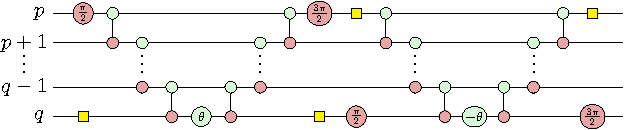
\includegraphics[width=14cm]{chapter-3/full_cnot}
\end{figure}

By defining the ordering of spin-orbitals such that adjacent spin-orbitals share the same spatial orbital, adjacent single-body operators commute.

\begin{equation*}
    \left[ \hat\kappa_p^q, \hat\kappa_{p+1}^{q+1} \right] = 0
\end{equation*}\smallskip

The same is therefore true for the resulting qubit operators,

\begin{equation*}
\begin{gathered}
    \left[ F_p^q, F_{p+1}^{q+1} \right] = 0 \\
    p, q \in \text{even} \qquad p+1, q+1 \in \text{odd}
\end{gathered}
\end{equation*}

This allows us to define the parametrised unitary qubit operators in terms of spin-adapted excitation operators.

\begin{equation*}
    U^q_p (\theta) = \text{exp}
    \left[ \theta \left( F_p^q + F_{p+1}^{q+1} \right) \right]
\end{equation*}

In other words, since $F_p^q$ and $F_{p+1}^{q+1}$ commute, we can think of them as a single operator with a single parameter.




